% ---------------------------------------------------------------------------
% Cosyne 2027 two-page extended abstract (deadline 18 October 2026).
%
% Format rules (cosyne.org/abstracts-submission, read 8 Oct 2026):
%   * two-page PDF, US Letter or A4, margins >= 0.5 in
%   * body font >= 12 pt; figure captions and references may be 10 pt
%   * title <= 100 characters incl. spaces, sentence case
%   * a <= 300-word summary (also pasted into a text-only box on the
%     submission site; it is the only text published in the program and
%     cannot be revised afterwards) followed by "additional detail"
%     (question, approach, results, conclusions; figures and equations
%     encouraged).  Reviewers see only this PDF.
%   * double blind: no names, affiliations, acknowledgments, or author
%     metadata; cite our own work in the third person ("[1]").
%   * pages beyond two are removed; non-compliant PDFs may be desk-rejected.
% There is no official template.  This file is self-contained and compiles
% with pdfLaTeX (no BibTeX needed: the reference list is written by hand).
%
% Version 3 = version 2 + slide-style reading of the norm inflation:
% the four terms of V (E_gen, sigma^2, n, T) and the three pieces of T_F
% (shrinkage weight, gradient Euclidean norm, gradient energy under Sigma)
% are colour-boxed in the equations, the interpretation paragraph walks
% through them, and the Significance paragraph turns each term into a
% remedy ("how to improve control").  Colours are defined once below;
% set \colorboxestrue/false to switch the boxes off for a plain build.
%
% Version 2 (mean/fluctuation structure).  Instead of following the paper's
% order (pixel ridge -> linear feature -> nonlinear feature), the body is
% organised around one decomposition: fitted weight = shrunk mean (safe:
% under-prediction only) + fluctuation (dangerous: norm inflation V ->
% over-prediction -> negative R^2).  All three settings then differ only in
% the gradient-geometry factor T inside V, which is interpreted as "which
% features are cheap or expensive for control".
%
% Figure plan.  Both figures are STAND-INS (paper figures squeezed into a
% dashed box of the intended footprint); remake offline at the stated size.
%   Fig 1 (full width x 1.7 in)
%     A  closed-loop paradigm: fit encoding model -> accentuate -> present
%     B  neural: (i) matched held-out prediction, (ii) two models' images
%        from one seed, (iii) self vs peer-review slope / R^2
%     C  linear teacher-student recapitulation of (i)-(iii)
%     D  equal-error geometry in the (high-PC, low-PC) weight plane:
%        prediction ellipsoids, control spheres, ridge path
%   Fig 2 (full width x 1.5 in)
%     A  NEW: mean vs fluctuation along the ridge path on van Hateren:
%        N=B11, |mean|^2=B22 and D=B22+V versus kappa (DE lines, MC markers),
%        with the CV penalty marked; below or inset, slope and R^2_acc for
%        the mean alone (safe) and for the full fit (crosses the R^2=0 cliff)
%     B  gauge rotation of the top-500-PC map: E_gen flat, T_F and R^2_acc move
%     C  neural: site-centred control slope vs log10 T_phi (r=-0.61) + bar of
%        -r for held-out MSE vs T_phi across 10/9/8/7-model subsets
% ---------------------------------------------------------------------------
\documentclass[12pt,letterpaper]{article}
\usepackage[margin=0.55in]{geometry}
\usepackage[T1]{fontenc}
\usepackage{times}
\usepackage{amsmath,amssymb,bm}
\usepackage{graphicx}
\usepackage{caption}
\usepackage[hidelinks]{hyperref}
\usepackage{xcolor}
% term colours (match the talk slides): noise/data terms in blues, geometry in salmon
\definecolor{cgen}{RGB}{204,222,236}   % E_gen
\definecolor{cnoise}{RGB}{196,226,230} % sigma^2
\definecolor{cdata}{RGB}{212,220,238}  % n
\definecolor{cgeo}{RGB}{250,214,204}   % T (gradient geometry)
\definecolor{cshrink}{RGB}{240,216,240}% shrinkage weight inside T
\definecolor{cnorm}{RGB}{232,232,232}  % gradient Euclidean norm
\definecolor{ccov}{RGB}{214,240,214}   % gradient energy under Sigma
\newif\ifcolorboxes\colorboxestrue
\newcommand{\hl}[2]{\ifcolorboxes{\setlength{\fboxsep}{1.2pt}\colorbox{#1}{$\displaystyle#2$}}\else#2\fi}
\newcommand{\hlt}[2]{\ifcolorboxes{\setlength{\fboxsep}{1pt}\colorbox{#1}{#2}}\else#2\fi}
\hypersetup{pdftitle={When good brain predictors make bad brain controllers: a regression theory of neural control},
            pdfauthor={},pdfsubject={Cosyne 2027 abstract (v3)},pdfkeywords={}}

\pagestyle{empty}
\setlength{\parindent}{0pt}
\setlength{\parskip}{1.5pt plus 1pt minus 1pt}
\setlength{\emergencystretch}{2em}
\linespread{0.87}
\setlength{\abovedisplayskip}{3pt}\setlength{\belowdisplayskip}{3pt}
\setlength{\abovedisplayshortskip}{2pt}\setlength{\belowdisplayshortskip}{2pt}
\captionsetup{font=footnotesize,labelfont=bf,labelsep=period,skip=2pt}  % footnotesize = 10 pt at 12 pt base
\setlength{\textfloatsep}{5pt}\setlength{\intextsep}{5pt}
% run-in bold headings
% (needspace-style guard so a heading is not stranded at a page bottom)
\newcommand{\runsection}[1]{\par\vskip0pt plus 3\baselineskip\penalty-100\vskip0pt plus -3\baselineskip\vspace{1.5pt}\noindent\textbf{#1}\hspace{0.5em}\ignorespaces}
% stand-in figure box: fixed footprint, dashed frame
\newcommand{\standin}[2]{\setlength{\fboxsep}{1pt}\setlength{\fboxrule}{0.3pt}%
  \fbox{\parbox[c][#1][c]{\dimexpr\linewidth-2\fboxsep-2\fboxrule}{\centering#2}}}
% non-floating figure: \placefig{height}{content}{caption}{label}
\newcommand{\placefig}[4]{\par\vspace{4pt}\noindent\begin{minipage}{\linewidth}\centering
  \standin{#1}{#2}\captionof{figure}{#3}\label{#4}\end{minipage}\par\vspace{4pt}}
% math
\newcommand{\x}{\mathbf{x}}
\newcommand{\bhat}{\hat{\beta}}
\newcommand{\bstar}{{\beta^{\star}}}
\newcommand{\bprime}{{\beta^{\prime}}}
\newcommand{\uvec}{\mathbf{u}}
\newcommand{\E}{\mathbb{E}}
\newcommand{\R}{\mathbb{R}}

\begin{document}

{\large\bfseries When good brain predictors make bad brain controllers: a regression theory of neural control\par}
\vspace{2pt}

% ---------------------------------------------------------------- summary (<= 300 words)
\textbf{Summary.}
Deep-network encoding models predict visual cortical responses to natural images so well that benchmarks can hardly rank them, and are increasingly used as controllers that synthesize images to drive a neuron to a target. A recent closed-loop benchmark of ten encoding models at 25 macaque V4/IT sites~[1] found that models with nearly identical held-out accuracy differed several-fold in control, that models which failed to control still recognized other models' successful images, and that control tracked the spatial-frequency content of a model's input gradient rather than its accuracy. We give a regression-theoretic account built on one decomposition. A fitted encoding weight is a mean, the true weight shrunk mode by mode by regularization, plus a zero-mean fluctuation from response noise and finite data. Prediction evaluates both in the metric of the natural-image covariance, where the fluctuation is nearly invisible. Control evaluates the model along its own gradient, in Euclidean geometry. There the mean is safe: shrinkage can only make the model under-predict its own stimuli. The fluctuation is not: it inflates the Euclidean norm of the weight without adding alignment to the neuron, so the model over-predicts its own stimuli, and once this norm inflation exceeds the shrinkage deficit, control $R^2$ turns negative. Peer review sees only the mean, explaining recognition without generation. Deterministic equivalents for ridge regression show that the inflation factorizes into a noise term, visible from held-out error, and a gradient-geometry factor that is not: the Euclidean energy of the model's well-resolved feature directions relative to their natural-image variance. Equally predictive feature maps differ in this factor without bound, cross-validation does not remove it, and its Jacobian version ranks deep encoding models by \emph{in vivo} control across 250 site--model pairs, where held-out accuracy carries none. Models must be validated on their gradients or generated stimuli, not prediction alone.

% ---------------------------------------------------------------- additional detail
\runsection{The phenomena.}
In the closed-loop paradigm of~[1] (Fig.~1A), responses of 25 V3/V4--IT sites in five macaques to ${\sim}1000$ naturalistic images were fit by cross-validated ridge regression on the features of ten deep-network backbones; each model then synthesized images by feature accentuation~[2] to drive its own prediction to graded targets, which were tested in a second session. Three observations motivate the theory (Fig.~1B). (i)~Models tightly matched on held-out images differed widely in the slope and $R^2$ between predicted and measured responses to their own images, often reaching the target with high-frequency texture that left the neuron unmoved. (ii)~In ``peer review'', a model whose own images failed still predicted responses to a successful model's images, often better than the generator. (iii)~Models whose input gradients concentrate power at low spatial frequencies controlled best. A linear teacher--student model on natural images reproduces (i)--(iii) (Fig.~1C).

\placefig{1.7in}{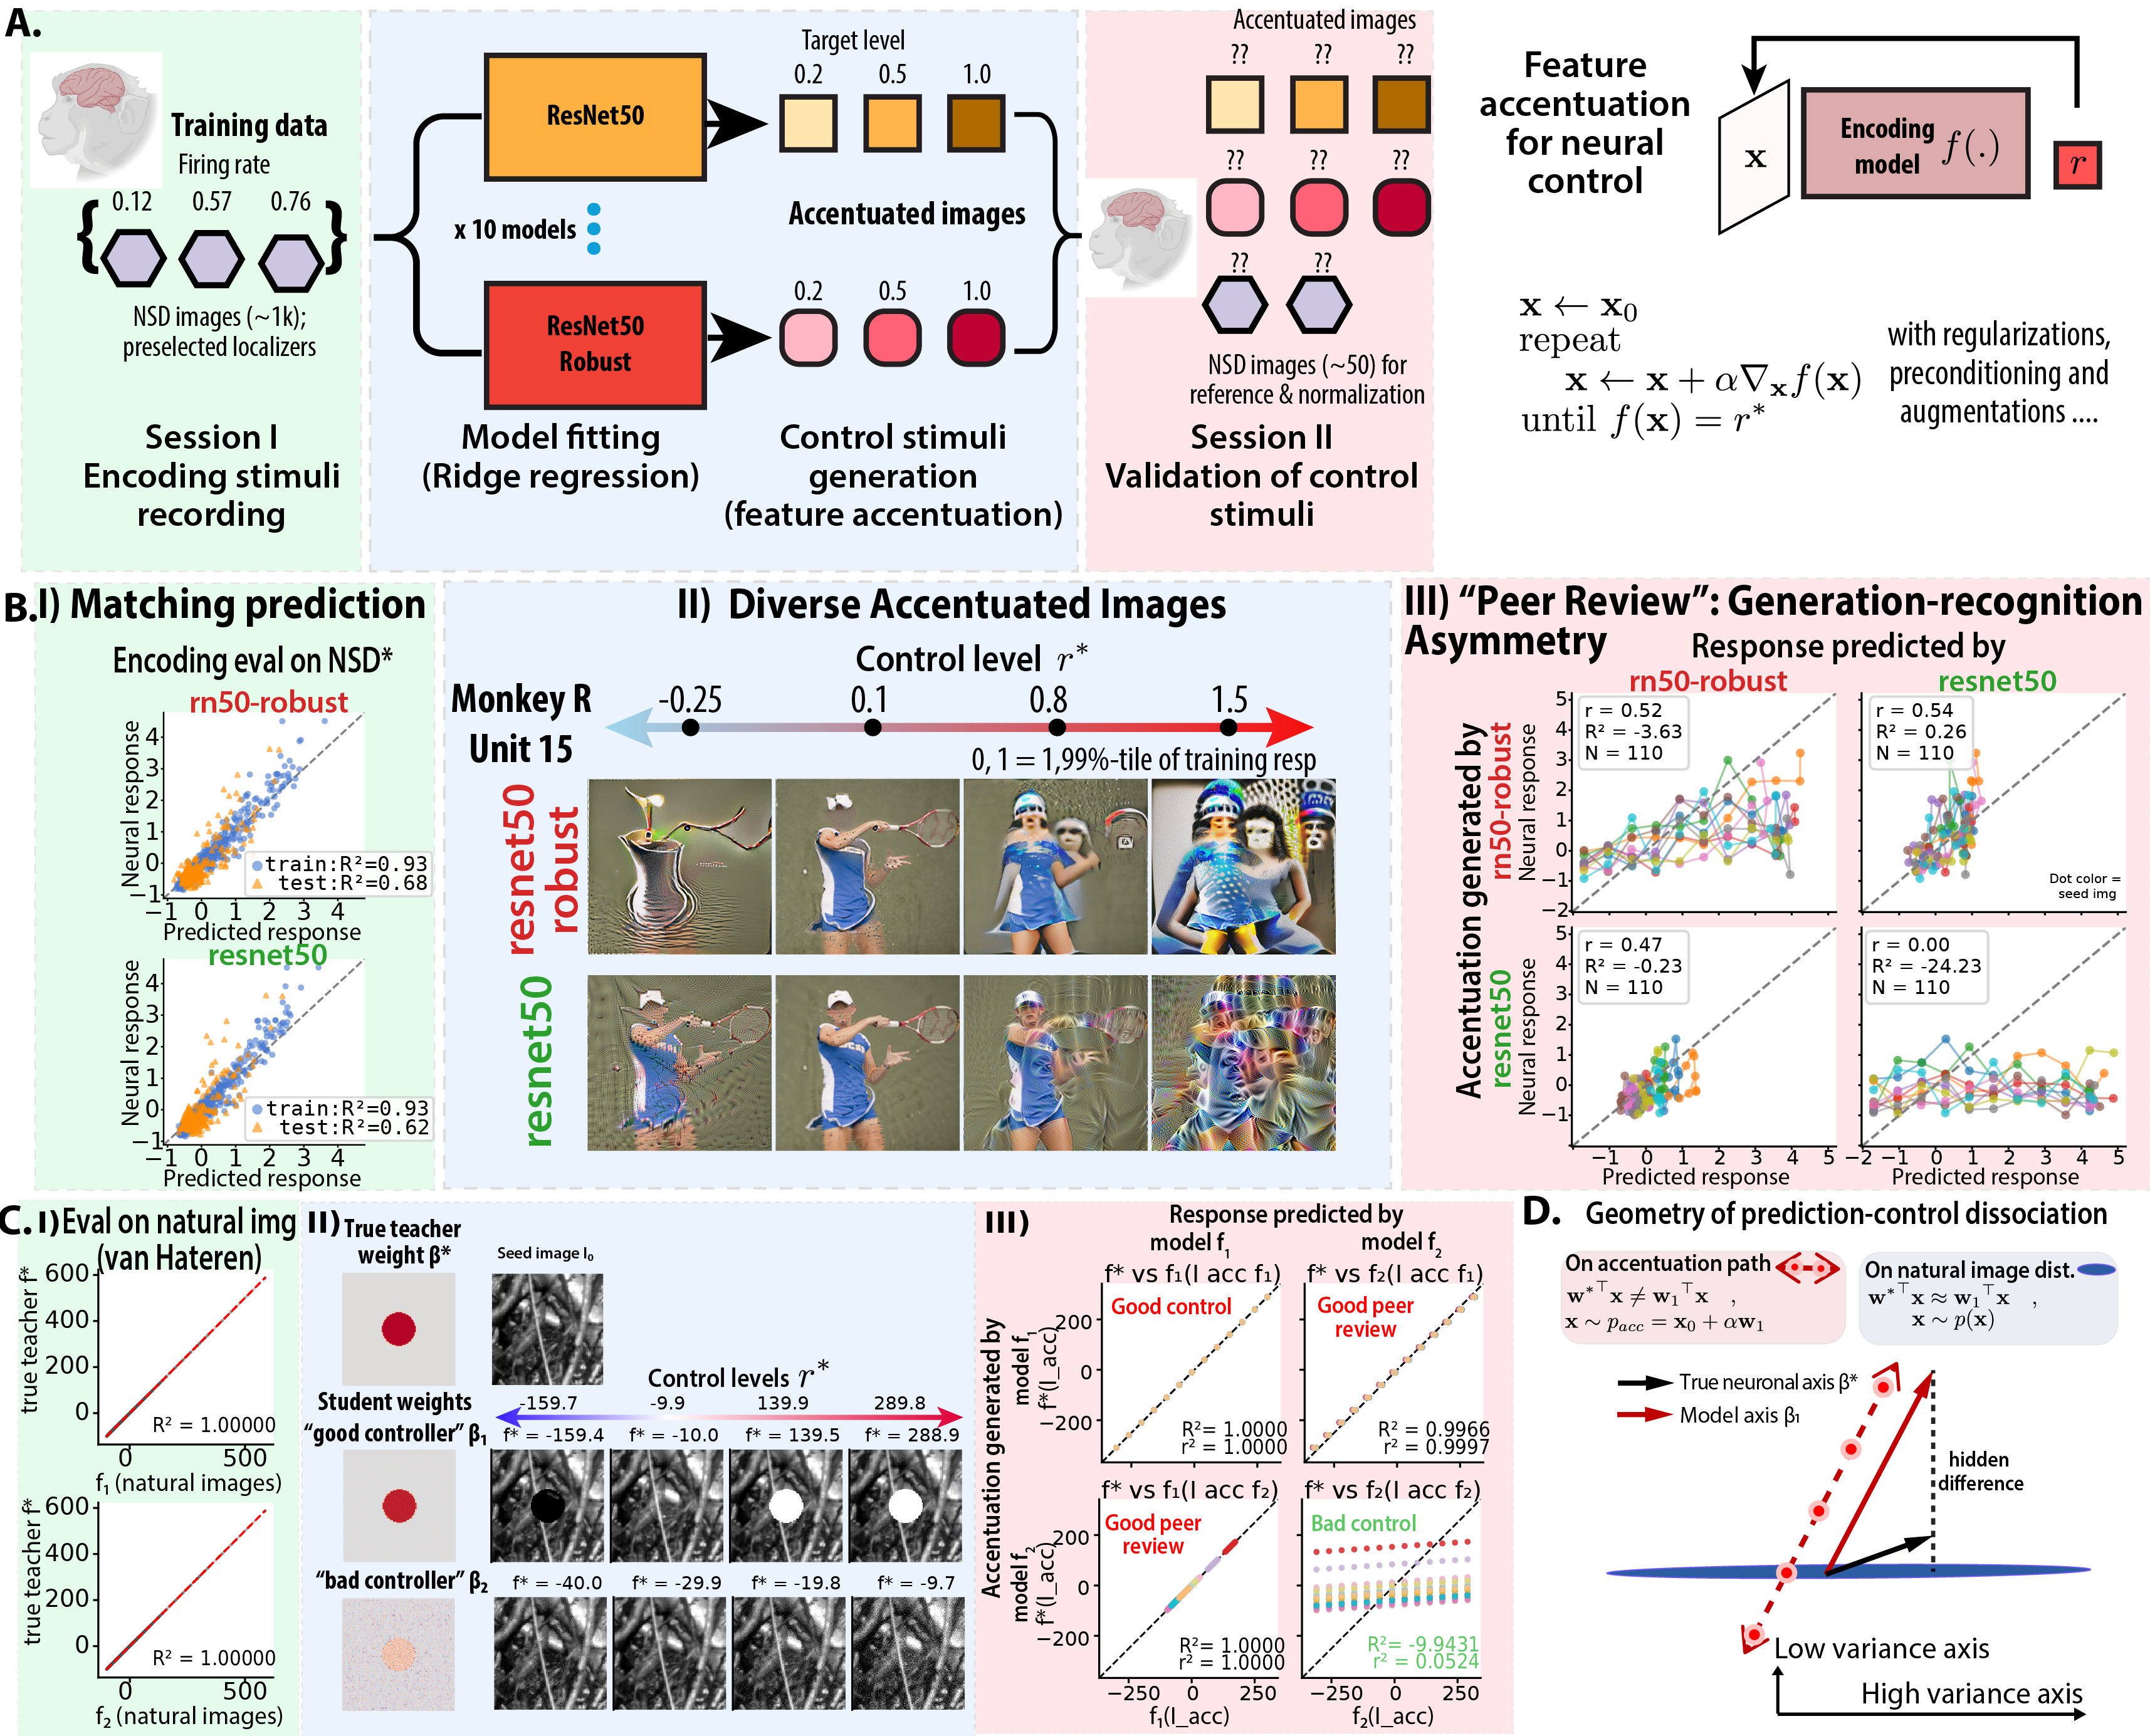
\includegraphics[height=1.65in]{figures/Figure_NeuroCtrl_results_Neuro-linear-compose.png}\hfill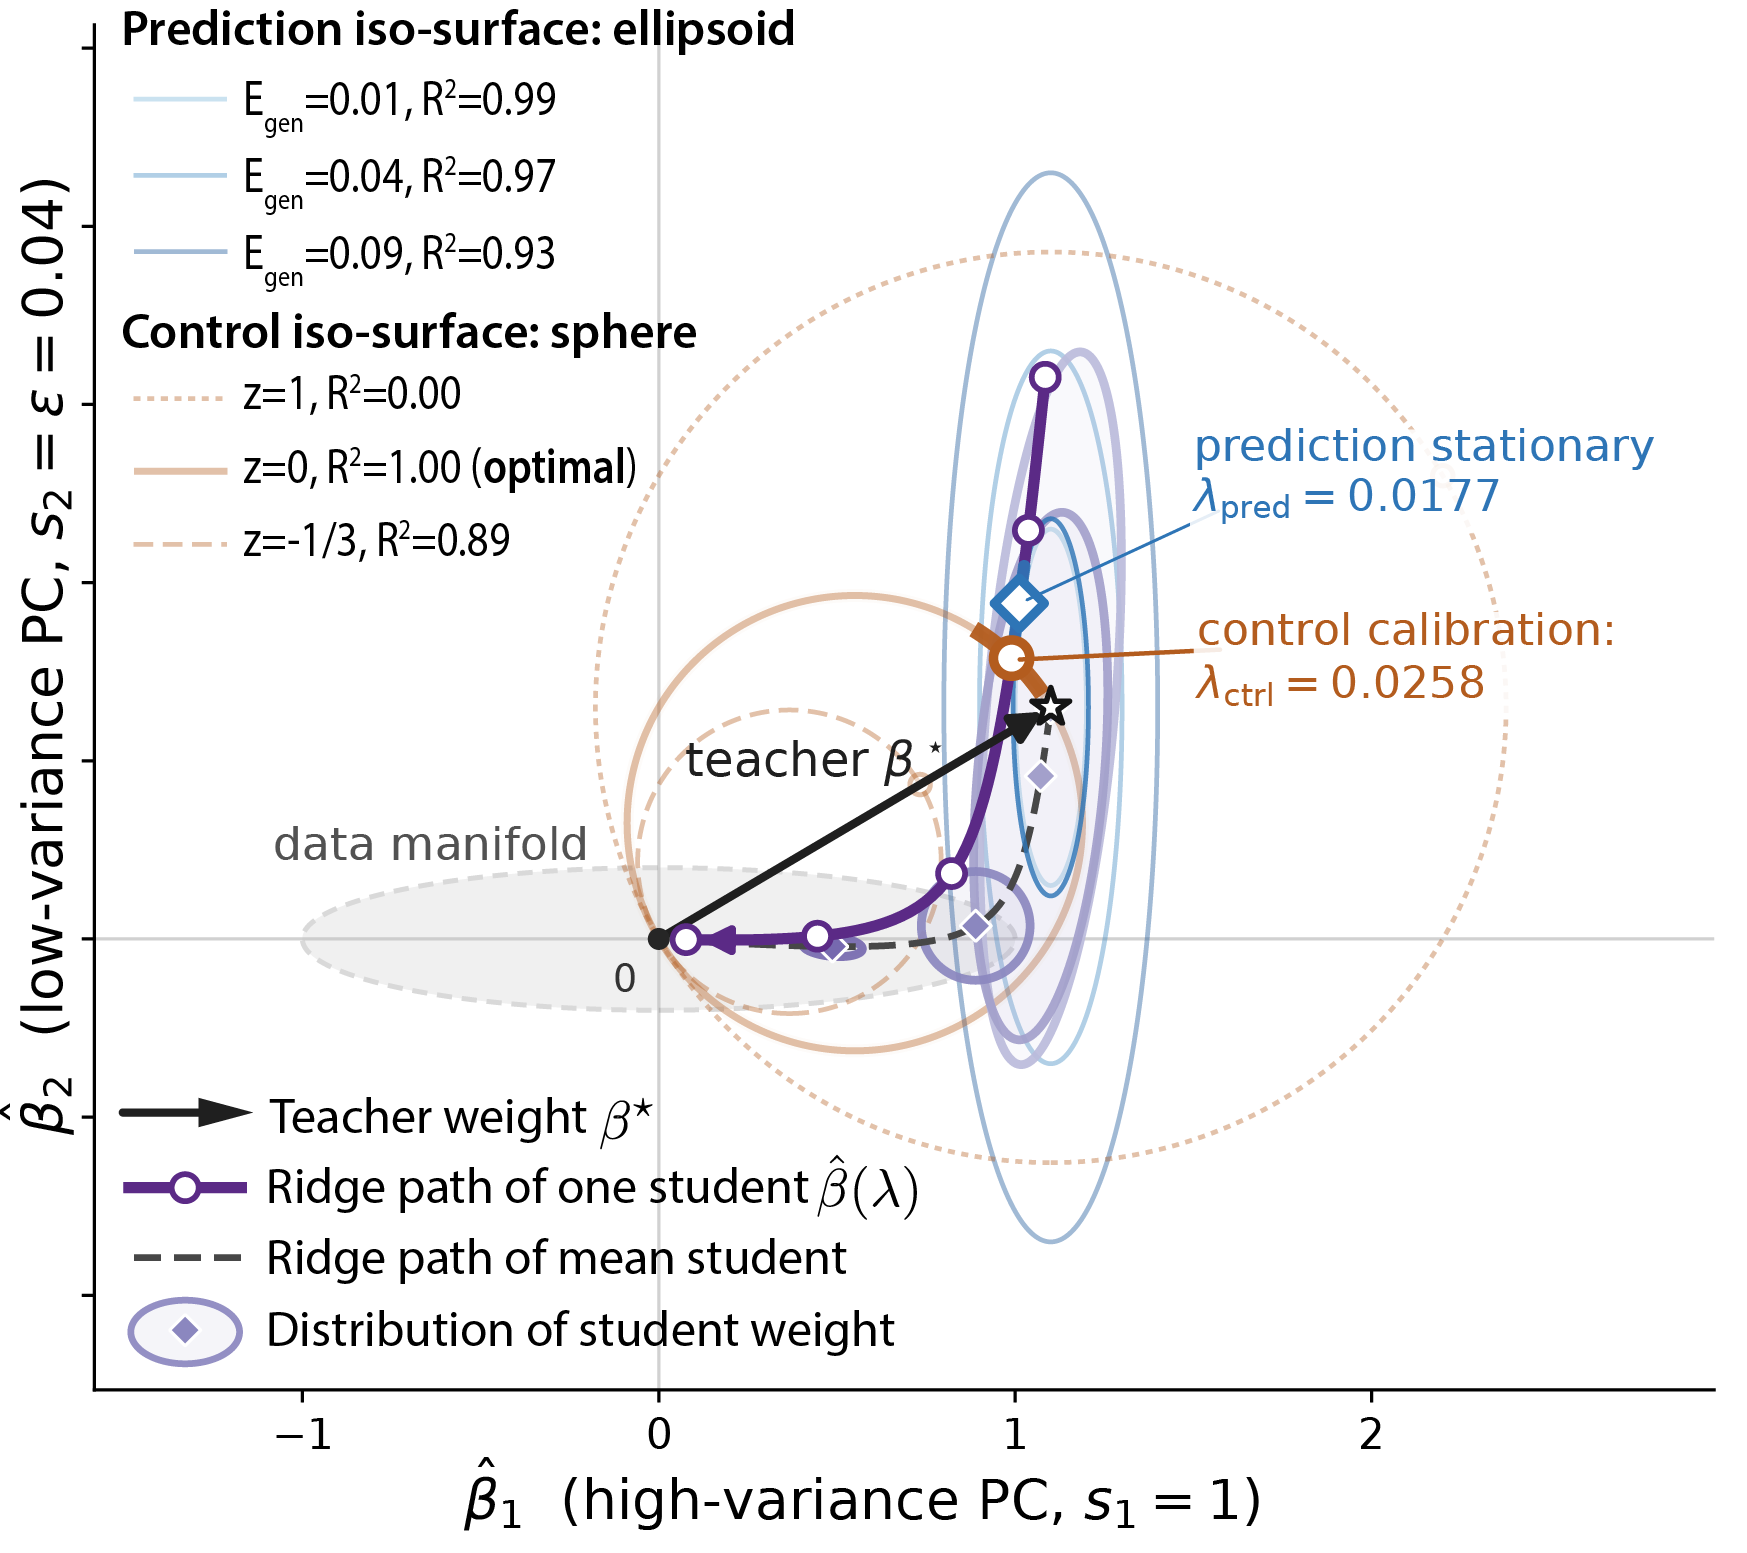
\includegraphics[height=1.65in]{figures/Figure_iso_err_surf_dissociation-01.png}}{\textbf{Prediction and control dissociate in neurons and in linear regression.}
\textbf{A}~Closed-loop paradigm of~[1]: encoding models fit to natural-image responses synthesize accentuated images that are tested in a second session.
\textbf{B}~Observations (i)--(iii) for two models.
\textbf{C}~Two linear students of one linear teacher, differing only along low-variance image directions, reproduce (i)--(iii).
\textbf{D}~Equal-error sets in the plane of a high- and a low-variance principal component: prediction ellipsoids, control spheres and the ridge path $\bhat(\lambda)$.}{fig:phenomena}

\runsection{Prediction is covariance-weighted, control is Euclidean.}
Idealize the neuron as a noisy linear teacher $y=\x^\top\bstar+\sigma\epsilon$ on inputs $\x\sim\mathcal N(0,\Sigma)$, $\Sigma=\sum_k s_k\uvec_k\uvec_k^\top$, and the model as a student $f(\x)=\x^\top\bhat$ fit from $n$ pairs. Held-out error is $E_{\rm gen}=(\bhat-\bstar)^\top\Sigma(\bhat-\bstar)$: an error along $\uvec_k$ costs $s_k$ times its squared length, so low-variance directions are nearly free. Accentuation moves along the model's own gradient, $\x=\alpha\bhat$, and every control metric is a function of one scalar, $z:=D/N-1$, with $N=\bhat^\top\bstar$ the alignment with the neuron and $D=\|\bhat\|^2$ the Euclidean norm: $\mathrm{slope}_{\rm acc}=1/(1+z)$, $R^2_{\rm acc}=1-z^2$. Equal-error sets in weight space are ellipsoids elongated along low-variance axes for prediction and Euclidean spheres for control (Fig.~1D); a student can sit deep inside a small ellipsoid yet on a huge sphere, which is how the students of Fig.~1C were built.

\runsection{A fitted weight is a safe mean plus a dangerous fluctuation.}
Ridge regression gives $\bhat=\bar\beta+\delta$: a mean $\bar\beta=\sum_k\frac{s_k}{s_k+\kappa}b_k\uvec_k$, the teacher $b_k=\uvec_k^\top\bstar$ shrunk mode by mode at the effective penalty $\kappa(\lambda)\ge\lambda$ of deterministic-equivalent theory~[3,4], plus a zero-mean fluctuation $\delta$ from response noise and the random design. Then
\begin{equation}\small
N\asymp\bstar^\top\bar\beta=B_{1,1},\qquad
D\asymp\|\bar\beta\|^2+V=B_{2,2}+V,\qquad V:=\E\|\delta\|^2,\qquad
\|\bstar\|^2\ge B_{1,1}\ge B_{2,2},
\label{eq:de}
\end{equation}
with $B_{p,q}=\sum_k s_k^pb_k^2/(s_k+\kappa)^q$. The mean alone gives $D\le N$: shrinkage makes the student \emph{under}-predict its own stimuli, with slope $\ge1$ and $R^2_{\rm acc}\in(0,1]$, never catastrophic. The fluctuation adds its Euclidean energy $V$, the \emph{norm inflation}, to $D$ but nothing to $N$: the student \emph{over}-predicts, and once $V$ exceeds the shrinkage deficit $B_{1,1}-B_{2,2}$, $z>0$ grows without bound and $R^2_{\rm acc}$ turns negative. Peer review sees only the mean, since independent fluctuations are uncorrelated: $\mathrm{slope}_{\rm peer}\asymp B_{1,1}/B_{2,2}\ge1$ and $R^2_{\rm peer}\ge0$, recognition without generation, with the signs seen in~[1] (self: median $R^2=-4.2$, slope $0.38$; peer: $0.04$, $1.35$).

\runsection{What sets the inflation: four factors.}
Deterministic equivalents give $V$ one form for ridge on a fixed linear feature map $F$ with feature-covariance eigenpairs $(s_k,v_k)$ (pixel regression is $F=I$) and, replacing $F$ by the Jacobian $J_\phi$, for a nonlinear map $\phi$:
\begin{equation}\small
V=\frac{\hl{cgeo}{T}}{\hl{cdata}{n}}\Big(\hl{cgen}{E_{\rm gen}}+\hl{cnoise}{\sigma^2}\Big),\quad
T_F=\sum_k\hl{cshrink}{\Big(\frac{s_k}{s_k+\kappa}\Big)^{\!2}}\frac{\hl{cnorm}{\|g_k\|^2}}{\hl{ccov}{g_k^\top\Sigma g_k}},\quad
T_\phi(x)=\sum_k\frac{s_k\|J_\phi(x)^\top v_k\|^2}{(s_k+\kappa)^2},
\label{eq:T}
\end{equation}
with $g_k=F^\top v_k$ the pixel gradient of feature PC $k$. Four factors inflate the norm: \hlt{cgen}{generalization error}, \hlt{cnoise}{observation noise}, \hlt{cdata}{limited data} and \hlt{cgeo}{gradient geometry $T$}. The first three are the noise level, which held-out error already reports; $T$ is a property of the feature map alone. It sums, over the \hlt{cshrink}{feature PCs surviving shrinkage} ($s_k\gtrsim\kappa$), the \hlt{cnorm}{Euclidean norm} of their pixel gradient relative to its \hlt{ccov}{natural-covariance energy}: control is most vulnerable when the top feature PCs backpropagate into the low-variance, high-spatial-frequency space of natural data (observation (iii)). Prediction cannot see $T$: held-out error and the cross-validated penalty depend on $F$ only through $\Sigma_F=F\Sigma F^\top$ and $F\Sigma\bstar$, which the maps $F\mapsto F\Sigma^{1/2}Q\Sigma^{-1/2}$ ($Q$ orthogonal, fixing $\Sigma^{1/2}\bstar$) preserve while moving $T_F$ and $R^2_{\rm acc}$ from near one to $-10^8$ (Fig.~2B). Nor does cross-validation remove the inflation: the prediction-optimal penalty minimizes $E_{\rm gen}$, not $|D-N|$, and on anisotropic images the two differ (Fig.~2A).

\placefig{1.5in}{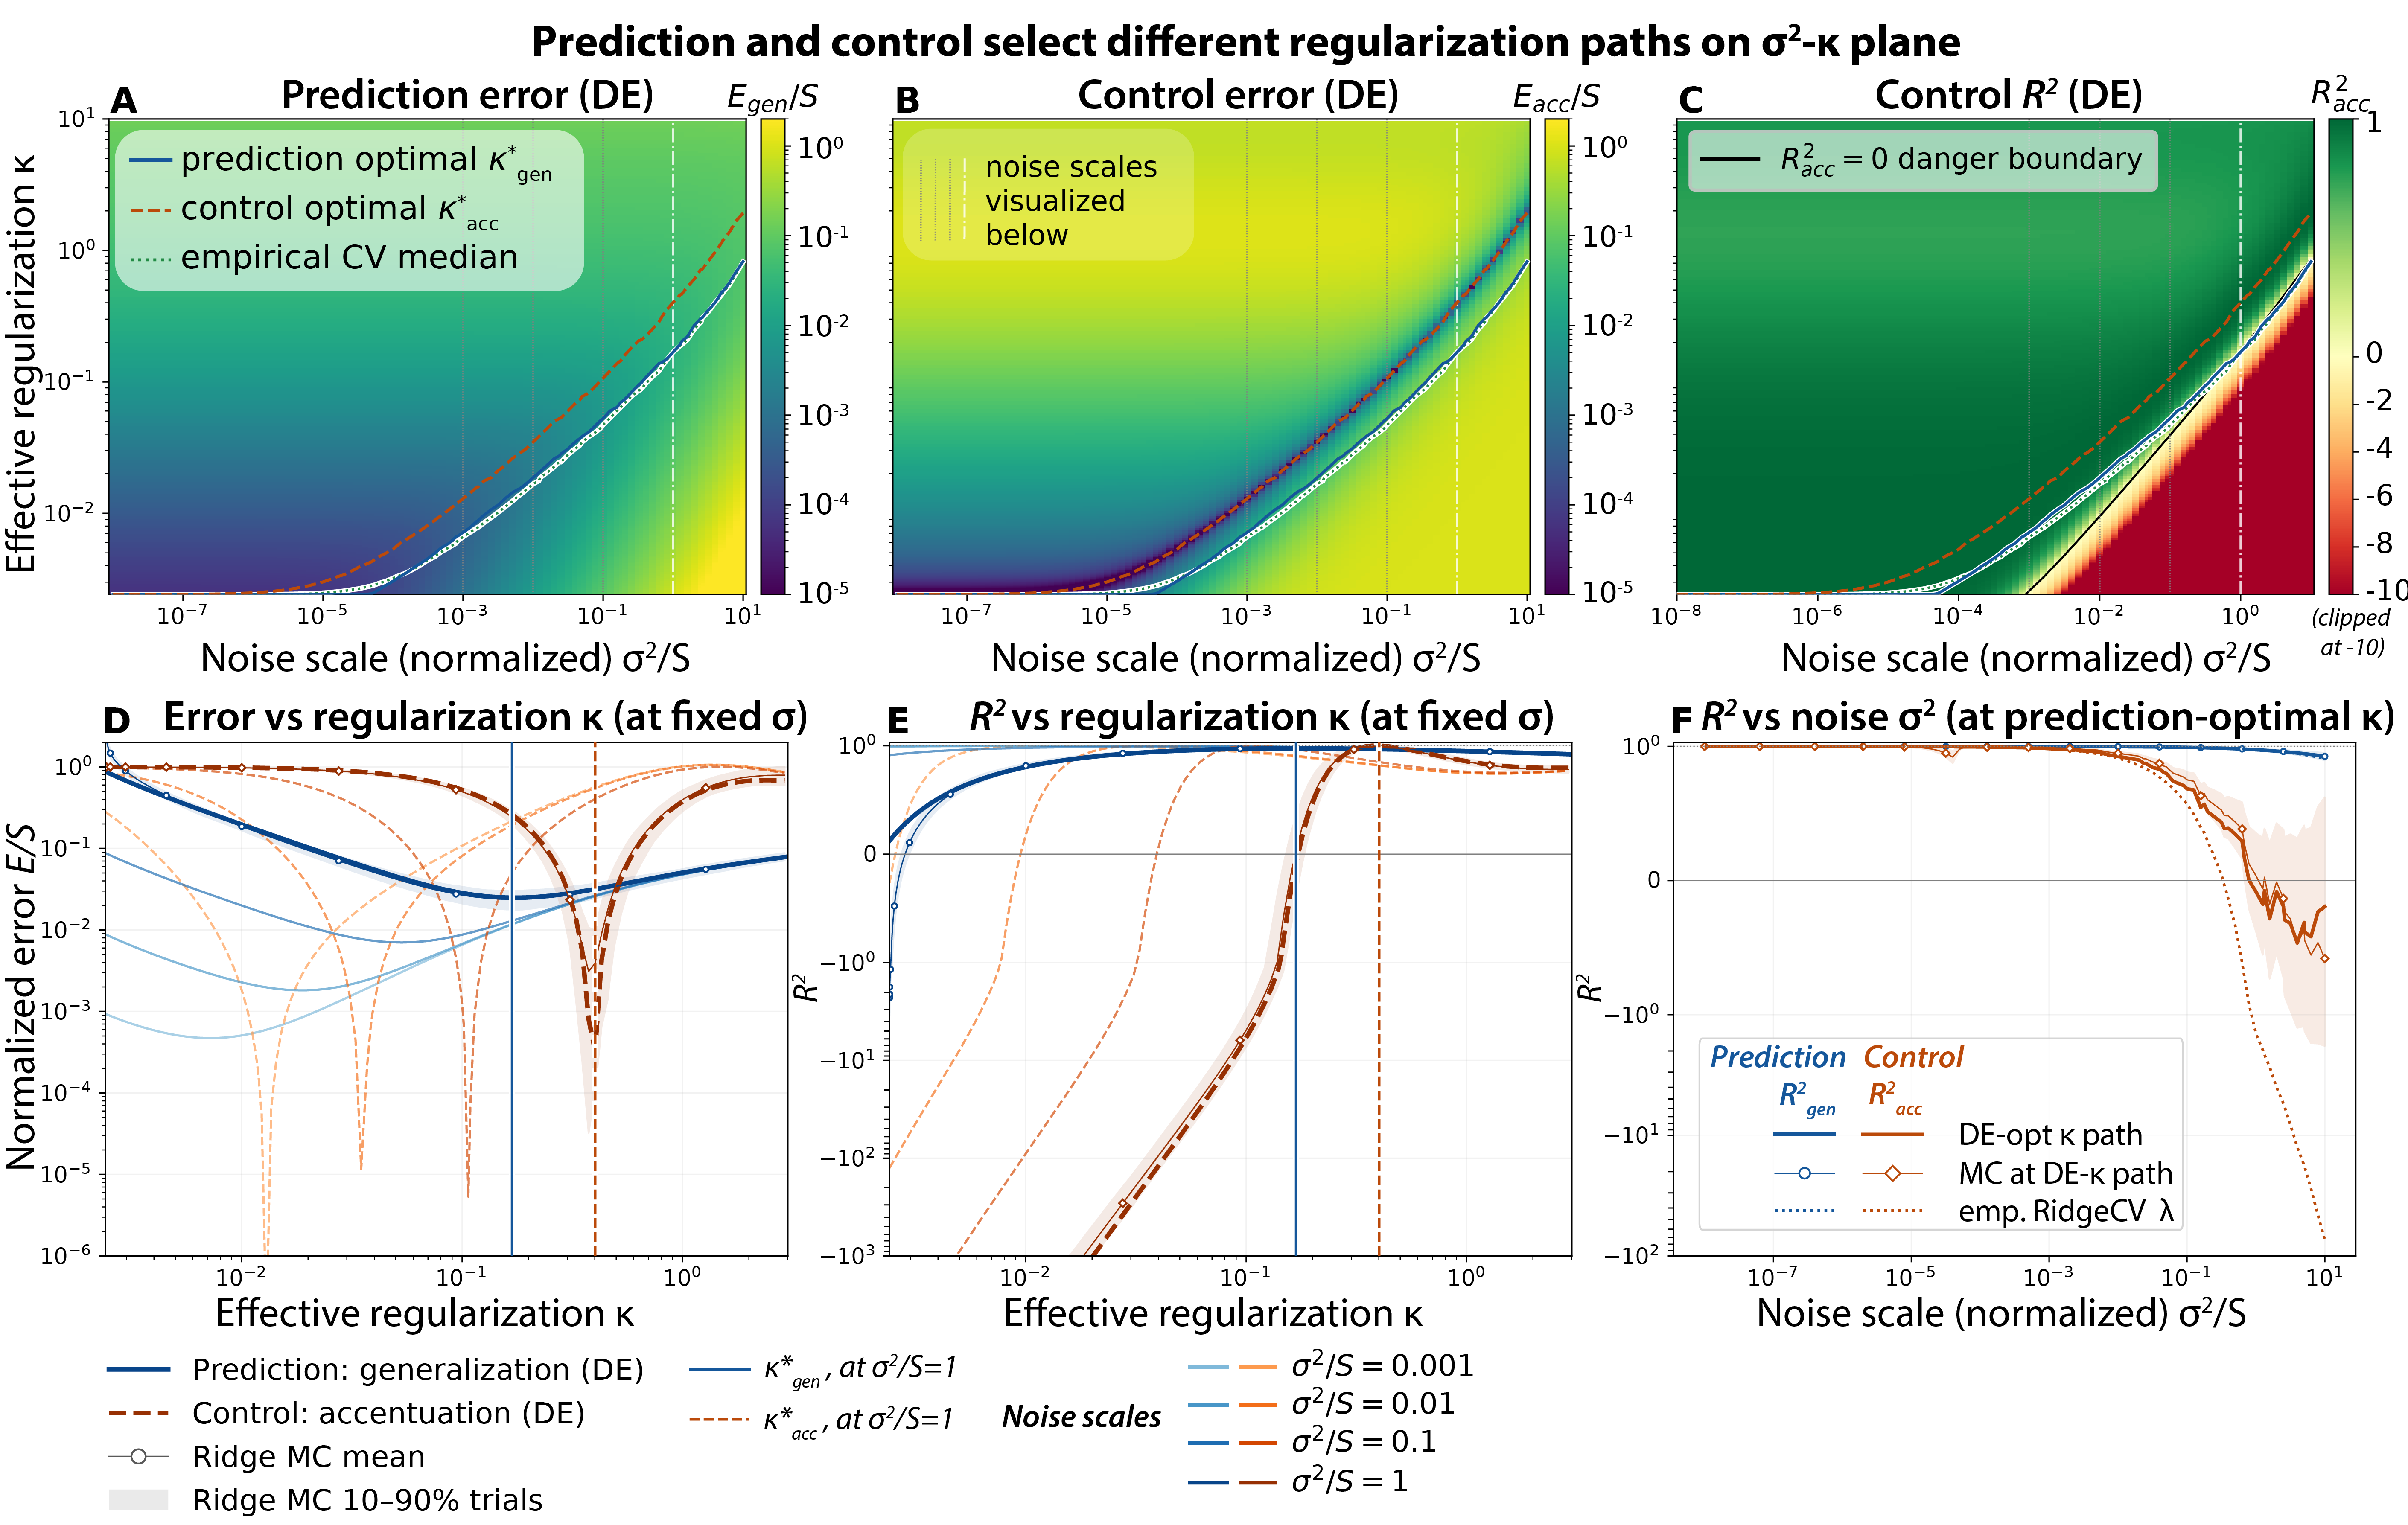
\includegraphics[width=0.5\linewidth,height=1.45in,keepaspectratio]{figures/Figure_PixRidgeGeometry.png}\hfill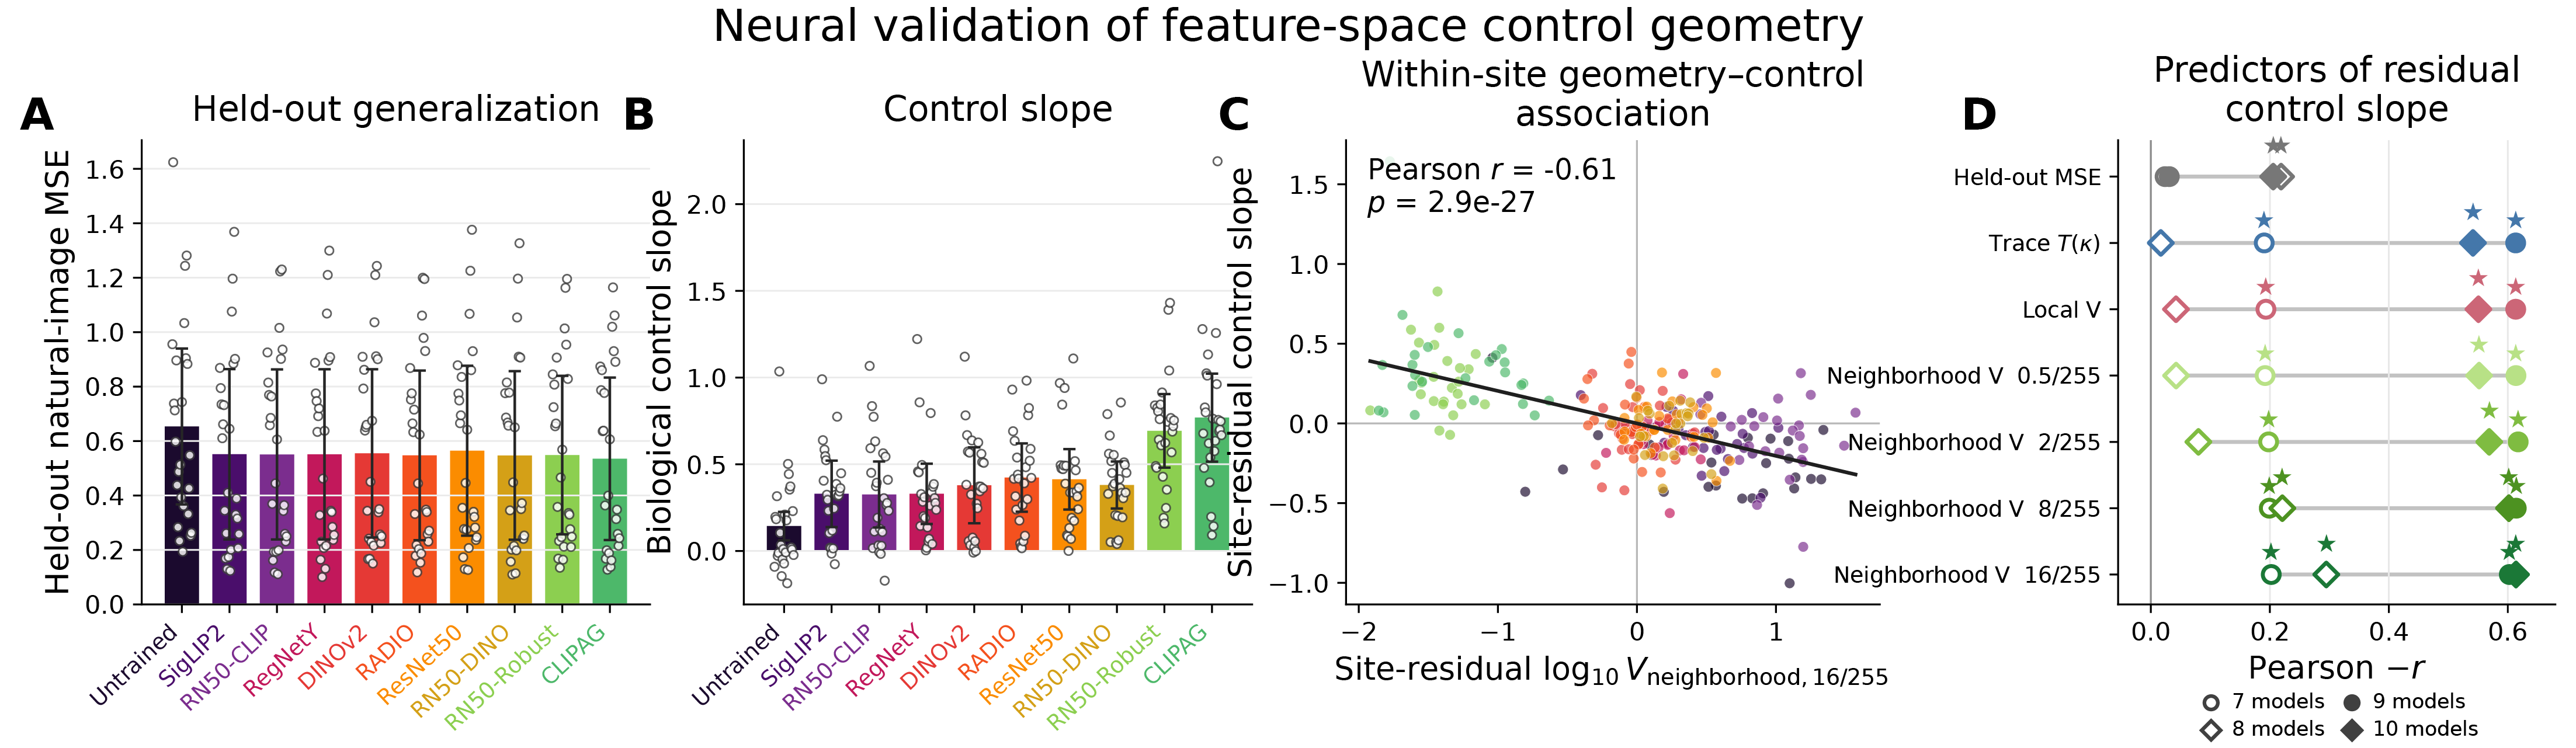
\includegraphics[width=0.48\linewidth,height=1.45in,keepaspectratio]{figures/Figure_nonlinear_neuro_diagnostic.png}}{\textbf{Mean, fluctuation and gradient geometry.}
\textbf{A}~Pixel ridge on van Hateren images along the penalty: $N$, mean norm $B_{2,2}$ and full norm $D=B_{2,2}+V$ (lines, theory; markers, Monte Carlo), and $R^2_{\rm acc}$ for the mean alone versus the full fit.
\textbf{B}~Prediction-preserving rotations of a top-500-PC feature map: $E_{\rm gen}$ constant while $T_F$ and $R^2_{\rm acc}$ move.
\textbf{C}~Neural data of~[1]: site-centred control slope against $\log_{10}T_\phi$ across 250 site--model pairs, and its correlation with held-out error versus $T_\phi$ for subsets of 10, 9, 8 and 7 models.}{fig:theory}

\runsection{Validation in silico and in vivo.}
On van Hateren images ($d=10^4$, $n=10^3$) theory tracks Monte Carlo, and the cross-validated student keeps $R^2_{\rm gen}$ high while $R^2_{\rm acc}$ turns strongly negative (Fig.~2A). Across the 250 site--model pairs of~[1], after site-centring, held-out error carries no ordering information (Pearson $r=0.02$ with control slope over nine trained models) whereas $T_\phi$ reaches $r=-0.61$ (Fig.~2C); the adversarially trained models, the strongest controllers, have the smallest $T_\phi$.

\runsection{Lesson: how to improve control.}
Each factor of $V$ names a remedy: better held-out \hlt{cgen}{prediction}, \hlt{cnoise}{denoising} or trial averaging, \hlt{cdata}{more images} to train on, and a backbone with \hlt{cgeo}{better gradients}, i.e.\ less power in low-variance data modes. Benchmarks address only the first; the last is invisible to them, yet it ordered the models \emph{in vivo} and is computable from $T_\phi$ before any experiment. Models should be validated on their gradients or generated stimuli, not on prediction alone.

% ---------------------------------------------------------------- references (10 pt, run-in, hand-written; numbers are hard-coded in the text)
\vspace{3pt}
{\fontsize{10}{10.5}\selectfont\setlength{\parskip}{0pt}\noindent\textbf{References.}
[1] Prince, Wang, et al. (2026). Parametric neural control differentiates top neural network models of primate visual cortex. \emph{bioRxiv}.
[2] Hamblin et al. (2024). Feature accentuation. \emph{arXiv:2402.10039}.
[3] Dobriban \& Wager (2018). High-dimensional asymptotics of prediction. \emph{Ann.\ Stat.}\ 46:247--279.
[4] Hastie et al. (2022). Surprises in high-dimensional ridgeless least squares interpolation. \emph{Ann.\ Stat.}\ 50:949--986.
[5] Bashivan, Kar \& DiCarlo (2019). Neural population control via deep image synthesis. \emph{Science} 364:eaav9436.\par}
\end{document}
